% \section{Results}
% \label{sec:result}
% In this section, we analyze and present the results from our data collection, which includes both sensor data and interview data.
% %
% First in \autoref{sec:result-overview-data},
% we provide an overview of the collected data, highlighting key statistics from the helmet-mounted sensors and enter/exit interviews.
% %
% Second in \autoref{sec:result-systemic},
% we analyze systemic patterns of air pollution and drivers' behaviors collected from the sensors.
% %
% Finally in \autoref{sec:result-individual},
% we integrate the sensor-collected data with interview insights to offer a more comprehensive understanding of the interplay between air pollution exposure and individual worker behavior.
% %
% % Finally in \autoref{sec:result-communal-engagement}, we describe how our online technical support messaging group has progressively evolved into a community space for the drivers to notify other drivers regarding potential air pollution hazards on a specific day and collectively strategizing their service routes.

\section{Overview of Collected Data}
\label{sec:result-overview-data}

\paragraph{Air Quality Data From Sensors}
Over the seven-month period (November 2023 to mid-May 2024), we collected data from ten motorcycle rideshare drivers in Bangkok and Chiang Mai, covering peak and non-peak pollution seasons.
Each driver wore a helmet-mounted low-cost PM2.5 sensor, calibrated against stationary PCD air quality towers in Chiang Mai and Bangkok.
In total, we captured over 50 million data points on street-level pollution in approximately 163.49 km$^2$ driven in Bangkok and 97.21 km$^2$ in downtown Chiang Mai.
Drivers drive approximately 6-10 hours per day, with consistent sensor functionality powered by portable power banks.



\paragraph{Exit Interviews}
We conducted qualitative exit interviews with all participants to supplement the sensor data. 
These interviews focused on understanding drivers' experiences with sensor-equipped helmets, their daily driving patterns, and any changes in awareness or behavior regarding air pollution. 
The author, a native Thai speaker, conducted the 60-90 minute interviews, using a semi-structured approach with open-ended questions. 

% \subsection{Systemic Patterns \joe{are these patterns "systematic"?}-- Aggregated Sensor Data Analysis}
\section{Results}
% \subsection{Aggregated Sensor Data Analysis}
% \label{sec:result-systemic}
% Aggregated Sensor Data Analysis
% (Examining the collective behaviors and patterns of all drivers through aggregated sensor data.)
% Analyzing overall driving behaviors and air quality exposure trends from sensor data.

% In this section, we analyze the collective behaviors of motorcycle taxi drivers through the air quality, location, and movement data from the helmet-mounted air-quality sensors.
% We aim to answer the following questions:
% \begin{enumerate}[label={\bf QS\arabic*}]
%     \item How is each driver exposed to PM 2.5 differently throughout different time periods?
%     \item How is each driver exposed to PM 2.5 differently throughout different parts of Bangkok and Chiang Mai?
%     % \item How is each driver exposed to PM 2.5 differently throughout both different parts of Bangkok and Chiang Mai and different periods of the study?
%     \item Based on the exposure patterns answered by the previous questions,
%     how do drivers respond as observed from the sensor data?
% \end{enumerate}
This section analyzes the collective behaviors of motorcycle taxi drivers using helmet-mounted sensor data (air quality, location, movement) to understand how individual PM2.5 exposure varies across time periods and locations, and how drivers subsequently respond based on these observed exposure patterns.

\begin{figure*}
    \centering
    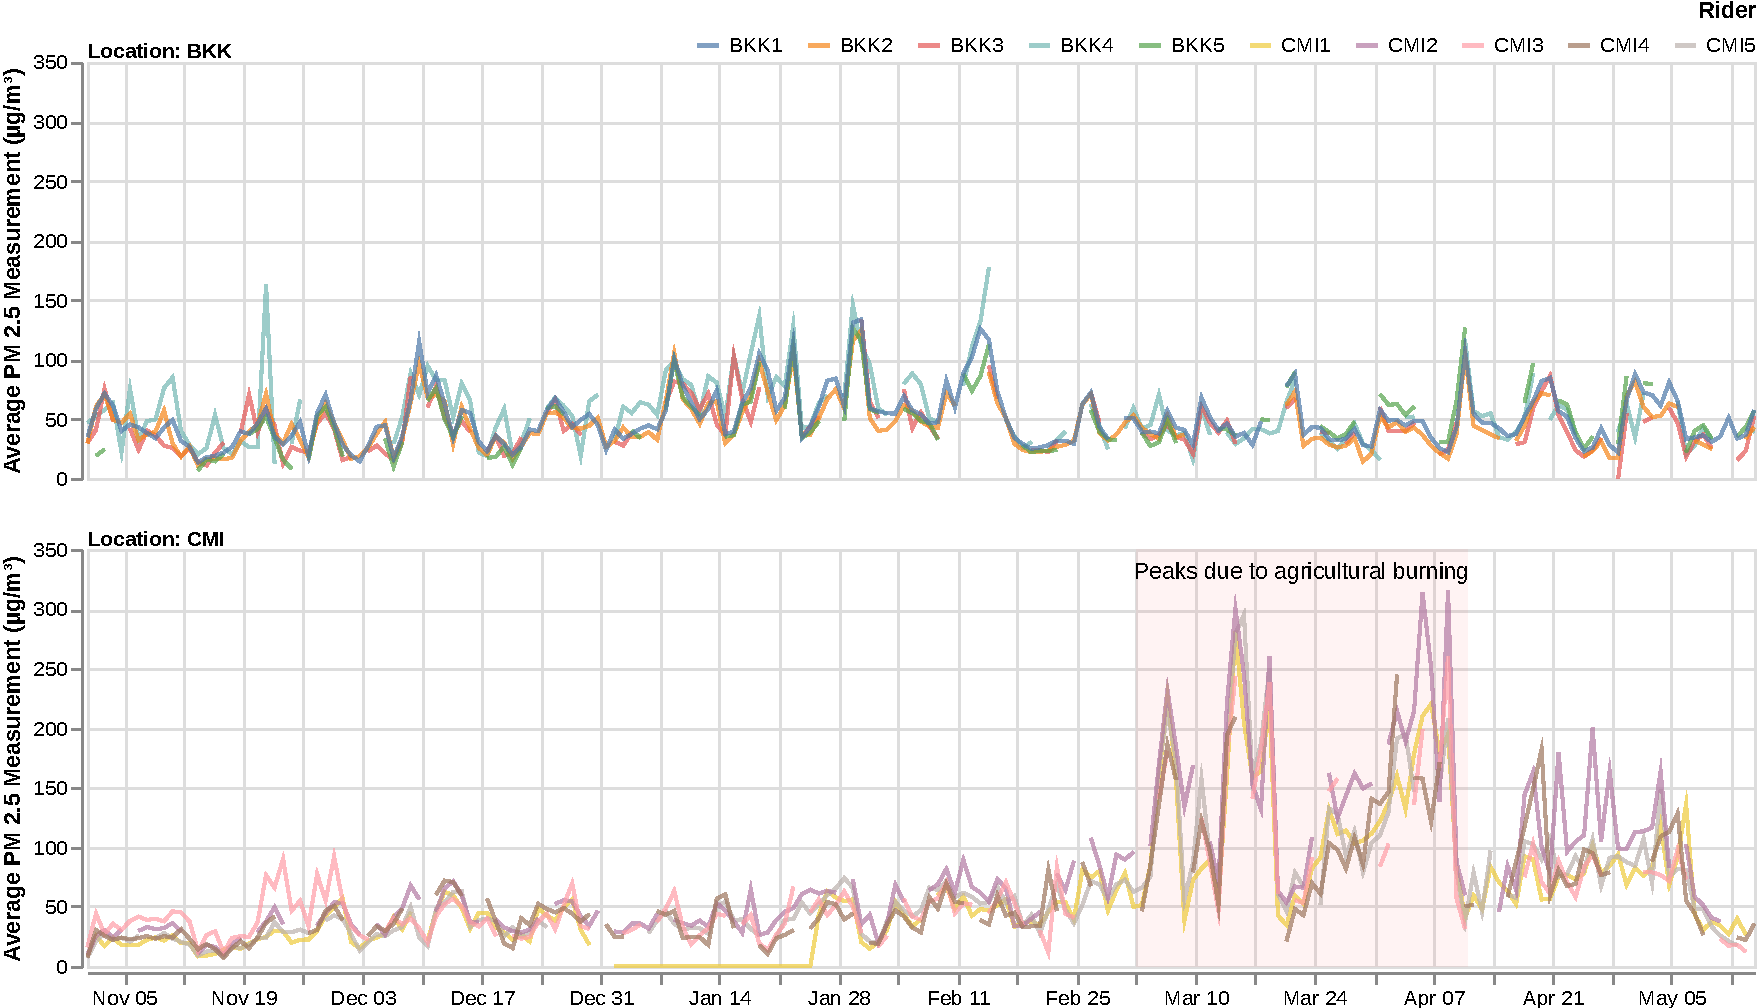
\includegraphics[width=\textwidth]{figures/daily-pollution-per-rider.pdf}
    \caption{
    Daily PM 2.5 exposure measured from the helmet-mounted sensors for Bangkok and Chiang Mai drivers.
    Vertical grid lines represent Sundays.
    }
    \Description{}
    \label{fig:daily-pollution-per-driver}
\end{figure*}

\subsection{PM2.5's Temporal Patterns}
Analyzing daily average PM2.5 exposure (\autoref{fig:daily-pollution-per-driver}) reveals relatively consistent levels in Bangkok (BKK), peaking moderately from December to mid-February,
while Chiang Mai (CMI) shows pronounced seasonality with extreme peaks from March to early April (consistent with agricultural burning periods~\cite{david2025chiangmaiburn, bernsten2024chiangmaiburn, iqair2023chiangmaiburn}).
% \joe{if you're going ot highlight it in the text like this, i would also highlight it in the figure}
Within each city, drivers experience similar daily trends.
Hourly averages (\autoref{fig:hourly-work-aqi}) show daily cycles peaking during morning (BKK: 7 AM, CMI: 8 AM) and evening rush hours, with an afternoon dip, although late night/early morning data shows higher variance.
Notably, BKK's PM2.5 measurements show a consistent trend throughout the year, reinforcing traffic as the primary air pollution source.
In contrast, CMI's dominant seasonal variation indicates agricultural burning as the primary driver.
Thus, PM2.5 sources differ substantially between cities (BKK: traffic, CMI: agricultural burning), implying the need for location-specific mitigation strategies.

% To find the PM 2.5 exposure amount of each driver throughout the different periods of the study,
% we present a relationship of the average amount of PM 2.5 measured from our sensor against days in the study in \autoref{fig:daily-pollution-per-driver}.
% We can see that the peak pollution in Bangkok is from December to mid-February; however, the amount of air pollution Bangkok drivers are exposed to is relatively consistent throughout the study period compared to that of Chiang Mai.
% On the other hand, PM 2.5 in Chiang Mai reaches high peaks from March to early April and low peaks afterward until May.
% We can attribute this consistency of the PM 2.5 level in Bangkok to its constant heavy traffic.
% In contrast, the condensed PM 2.5 peak period in Chiang Mai is consistent with yearly agricultural burning periods,
% which typically end in April,
% as evidenced by climate articles~\cite{david2025chiangmaiburn, bernsten2024chiangmaiburn, iqair2023chiangmaiburn}.
% % \mick{enforcement for agricultural burning}\footnote{\mick{\url{https://radiochiangmai.prd.go.th/th/content/category/detail/id/57/iid/352430}, \url{https://maesa.go.th/public/list/data/detail/id/5046/menu/1554}}}
% In addition, despite each driver's independence,
% all of the drivers in the study in each location still are exposed to the same amount of pollution, as shown in \autoref{fig:daily-pollution-per-driver}.

% To drill down into the finer-grain time period, we analyze PM 2.5 exposure patterns throughout each of the drivers' work days, as shown in \autoref{fig:hourly-work-aqi}.
% We can observe that the PM 2.5 exposure is consistently the highest at 7 AM for Bangkok and 8 AM for Chiang Mai, as these are both provinces' rush hours.
% The measurements for both provinces consistently slope down until the afternoon when they reach their lowest measurement values.
% The measurements climb back up again in the evening as workers travel back to their residents.
% The measurements collected at late night and early morning are inconsistent as indicated by the wider standard deviation range.
% % \mick{can we say here that because we have fewer data points -> less consistent?}
% The pattern with high PM 2.5 exposure during the morning and afternoon is less visible from March to May in Bangkok.
% This is the period when the majority of schools in Bangkok are on Summer break.
% The measured PM 2.5 patterns are highly correlated with Bangkok residents' commute behavior.
% This correlation further emphasizes that the primary source of PM 2.5 measured by Bangkok drivers is traffic pollution.
% On the other hand, in Chiang Mai, the measured PM 2.5 pattern with respect to months of the year is more prominent than patterns observed from measured PM 2.5 within a day.
% This indication leads us to conclude that the primary source of PM 2.5 measured by Chiang Mai drivers is agricultural burning.
% These results are also consistent with our analysis for \autoref{fig:daily-pollution-per-driver}.
% % \mick{can add analysis of PM 2.5 per day of the week if we have space.}

\begin{figure*}
    \centering
    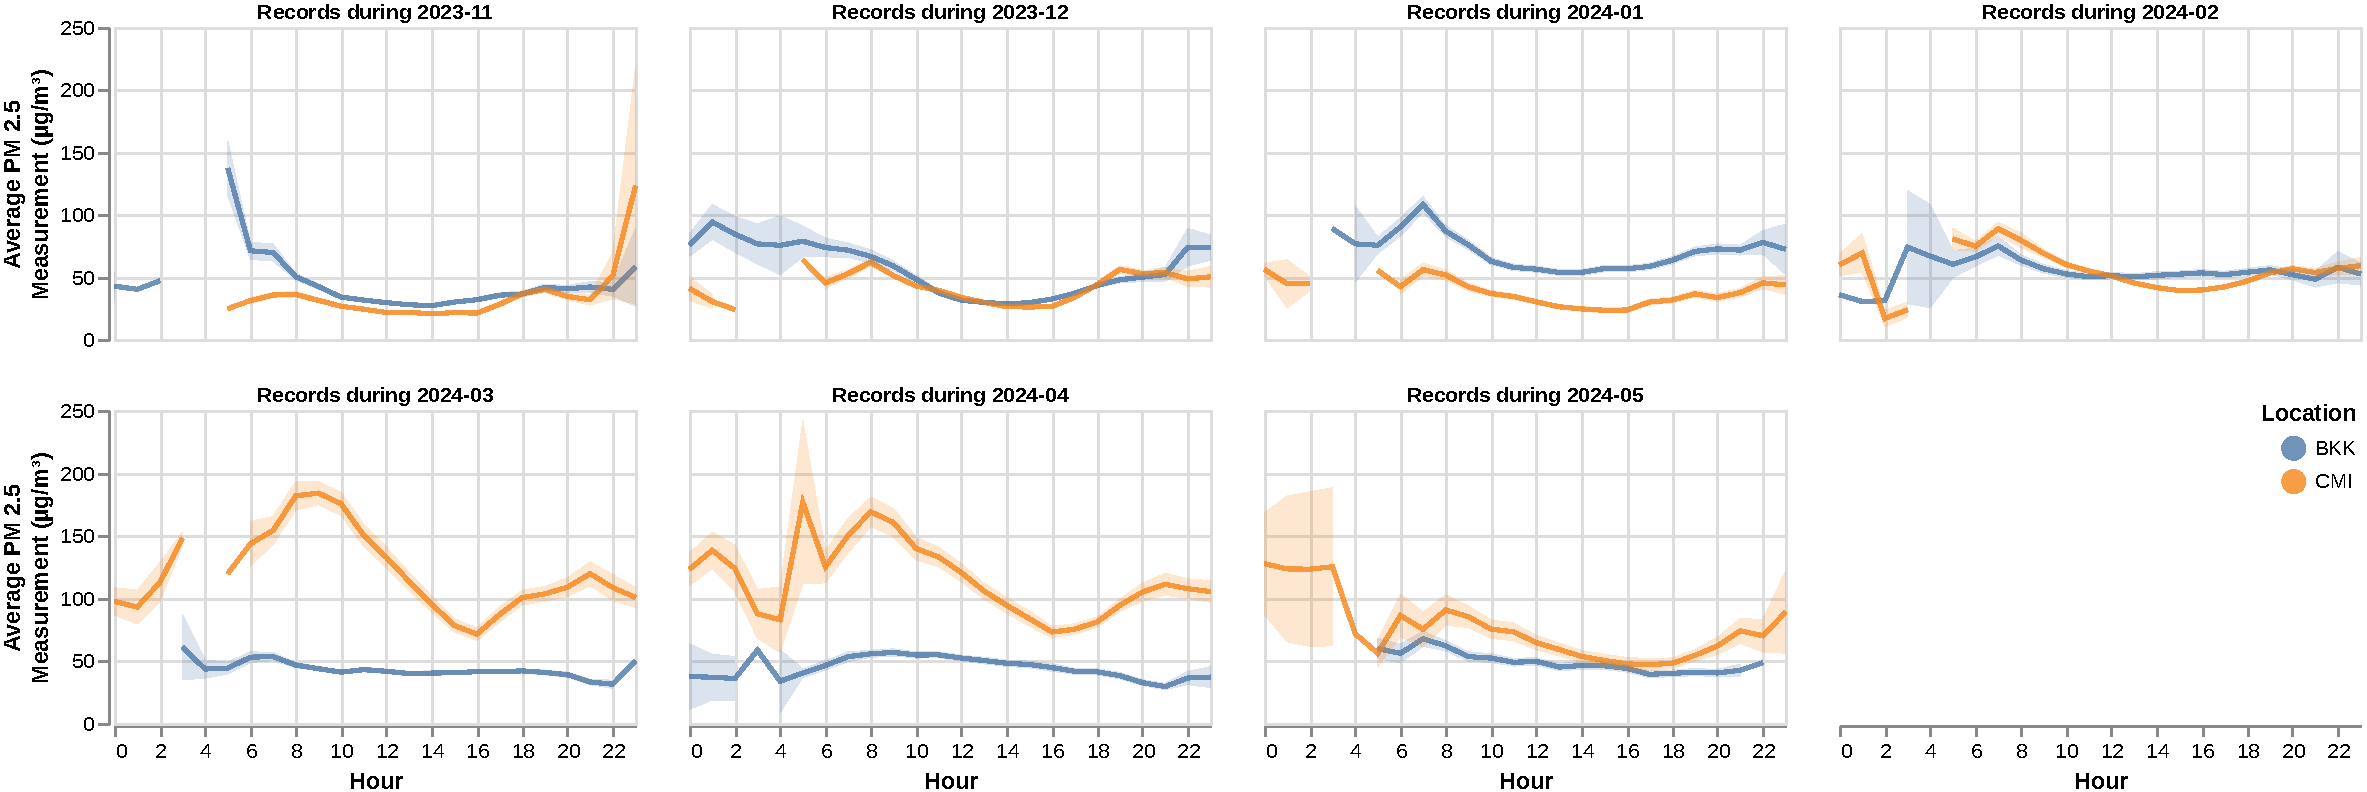
\includegraphics[width=\textwidth]{figures/average-hourly-pollution.pdf}%
    \caption{Mean and standard deviations of air pollution measurement in each hour of the day throughout the study period.
    % Each colored band represents $\pm1$ standard deviation from its average line. \joe{you can just say "mean and standard deviations shown" people know what fillbetween() represents.}
    Each subplot represents each month in the study. }%
    \Description{}
    \label{fig:hourly-work-aqi}%
\end{figure*}%

% % \begin{figure}
% %     \centering
% %     \begin{subfigure}[t]{0.49\textwidth}
% %         \centering
% %         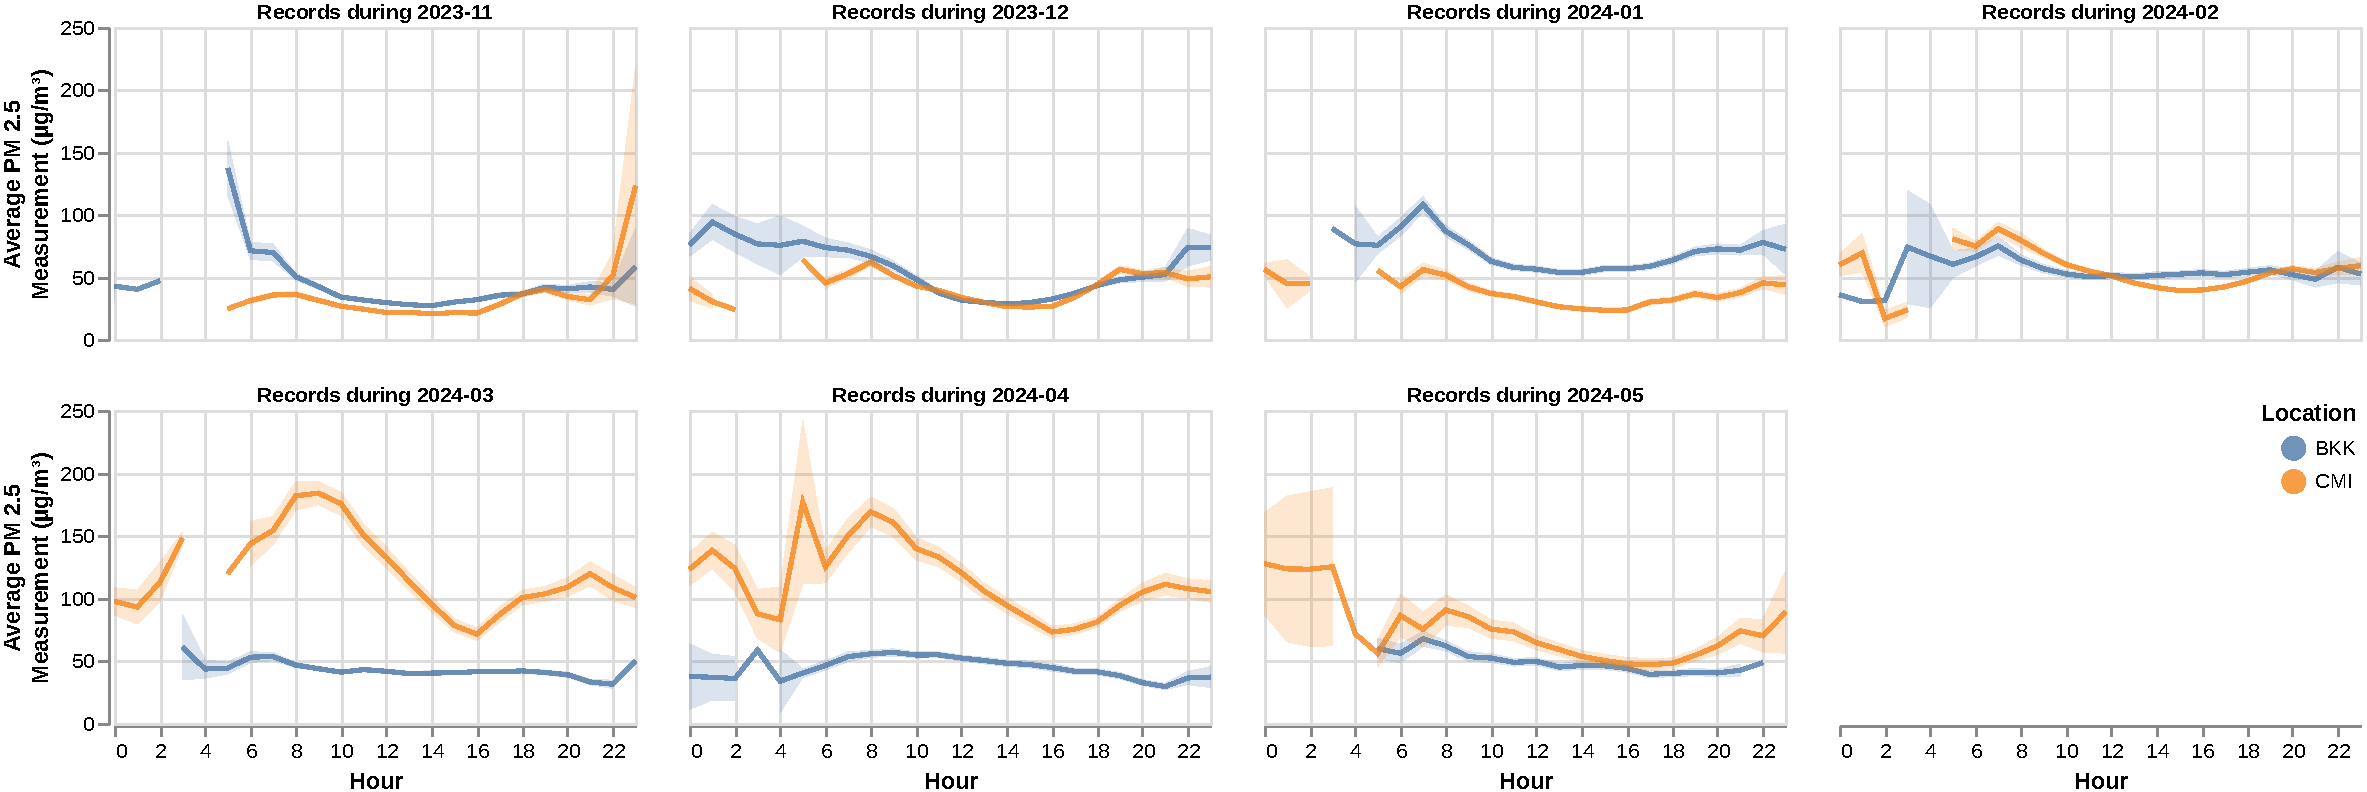
\includegraphics[width=\linewidth]{figures/average-hourly-pollution.pdf}%
% %         \caption{Average air pollution measurement in each hour of the day throughout the study period.}
% %         \label{fig:hourly-work-aqi}
% %     \end{subfigure}%
% %     \hfill%
% %     \begin{subfigure}[t]{0.49\textwidth}
% %         \centering
% %         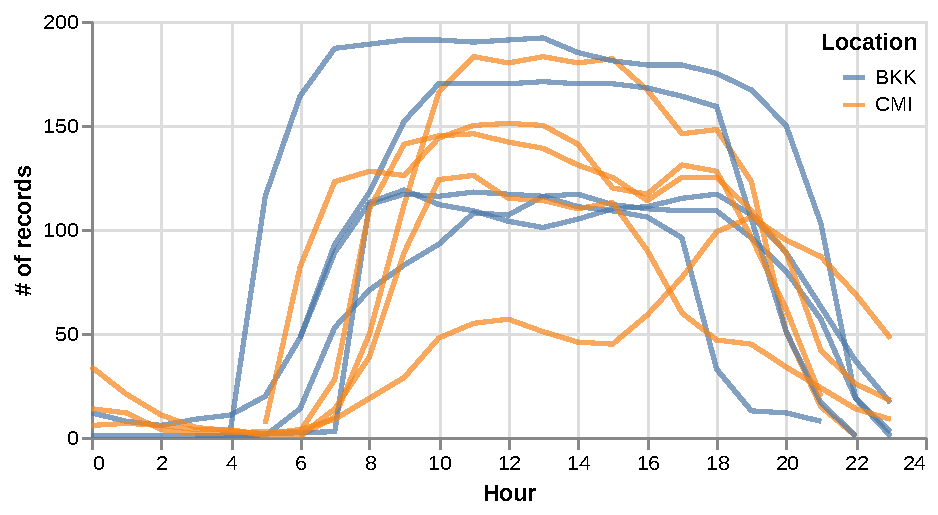
\includegraphics[width=\linewidth]{figures/hourly-records-per-location.pdf}%
% %         \caption{Number of records for each hour of the day throughout the study period. \mick{todo: divide by the \# of days they work}}
% %         \label{fig:hourly-work-hours}
% %     \end{subfigure}%
% %     \caption{
% %     Air pollution exposure and hour work for each hour of the day.
% %     \joe{shift x axis index by 1 so its not 0-23 but 1-24 for right plot and explain in text whether we actually have rider data from 22-3 as and how often. was it a few riders that drove at night?}
% %     }%
% %     \label{fig:hourly-work-stats}%
% % \end{figure}%

% % {\bf Answers to QS1.}
% \paragraph{Answers to QS1}
% % \mick{peaks at xxx; bkk is more consistent; chiang mai has lower pm 2.5 values during the normal period, but higher peaks; drivers seem to be exposed to similar amounts of PM 2.5 among drivers in the same province.}
% The PM 2.5 measured in Chiang Mai primarily follows the patterns of agricultural burning,
% while PM 2.5 measured in Bangkok primarily correlates with the commute behaviors of Bangkok residents and, thus, likely comes from traffic pollution.
% % \mick{the time granularity? for tackling AQ problem in each region are different (no one solution that fits regions)}
% As a result, the solution for lessening the amount of PM 2.5 exposed between both provinces must be different depending on the source of air pollution.

\subsection{PM2.5's Spatial Patterns}
% The results from analyzing the temporal patterns of PM 2.5 measurement indicate that participants in the same province are exposed to PM 2.5 at a similar amount at any given time throughout the study.
% In this section, we analyze the relationship between the amount of PM 2.5 measured and the locations of the drivers.
% As shown in \autoref{fig:subdistrict-aqi}, in each sub-figure, the plots in the right columns reveal that all of the drivers in the study mostly stay in one location. 
% The plots in the left columns also reveal that the PM 2.5 level is distributed unevenly across both provinces' subdistricts and drivers.

% \paragraph{Answer to QS2}
% The drivers experience different amounts of PM 2.5 even at the same approximate location.
% Each driver also spends the majority of their time at a different place.
% As a result, the solution for reducing the drivers' exposure to PM 2.5 should also take into account their active locations during their work.
Spatial analysis (\autoref{fig:subdistrict-aqi}) reveals that PM2.5 distribution is uneven across subdistricts and individual drivers, with drivers experiencing different exposure levels even in similar areas.
Furthermore, each driver tends to operate primarily within specific locations.
Consequently, effective PM2.5 exposure mitigation strategies must consider these individual spatial work patterns.
% \joe{is there openstreetmap in bangkok and chiangmai? can you compare the AQI with some environmental feature that you can pull from OSM? For example, number of intersections, width of roads, density of roads, etc. Would be cool to try to actually learn something about why AQI is worse in certain areas.}

\begin{figure*}
    \centering
    \begin{subfigure}[t]{0.49\textwidth}
        \centering
        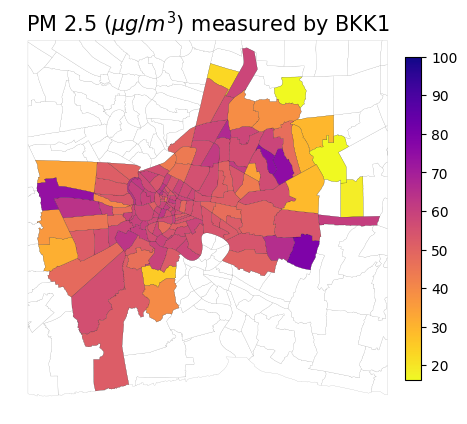
\includegraphics[width=.49\linewidth]{figures/map/BKK1_PM25.png}%
        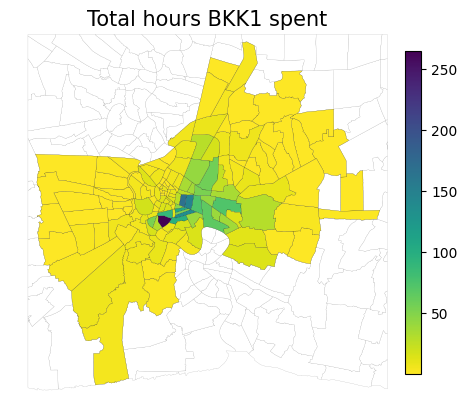
\includegraphics[width=.49\linewidth]{figures/map/BKK1_time.png}
        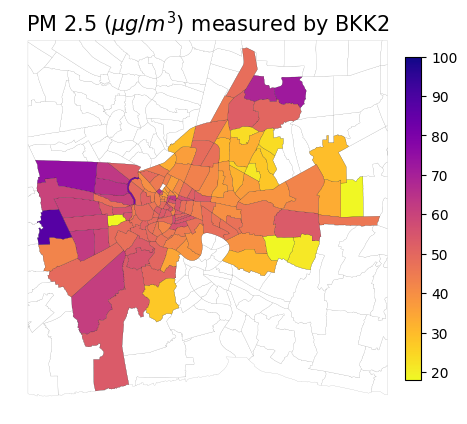
\includegraphics[width=.49\linewidth]{figures/map/BKK2_PM25.png}%
        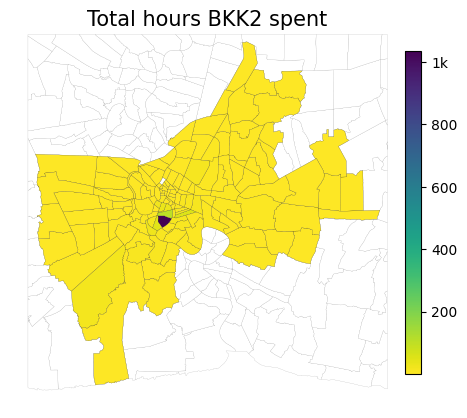
\includegraphics[width=.49\linewidth]{figures/map/BKK2_time.png}
        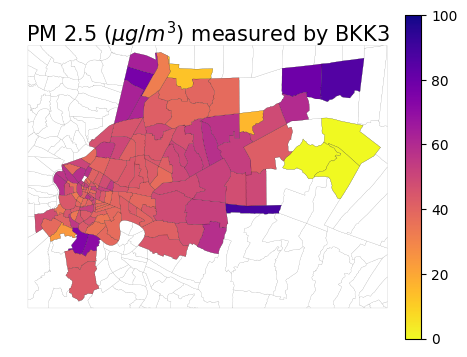
\includegraphics[width=.49\linewidth]{figures/map/BKK3_PM25.png}%
        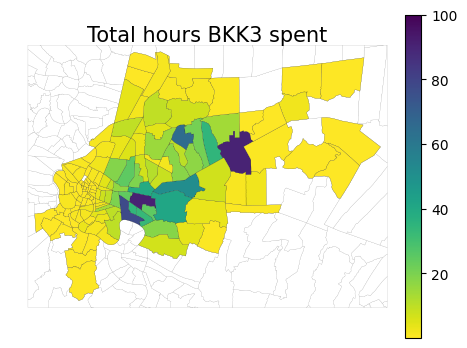
\includegraphics[width=.49\linewidth]{figures/map/BKK3_time.png}
        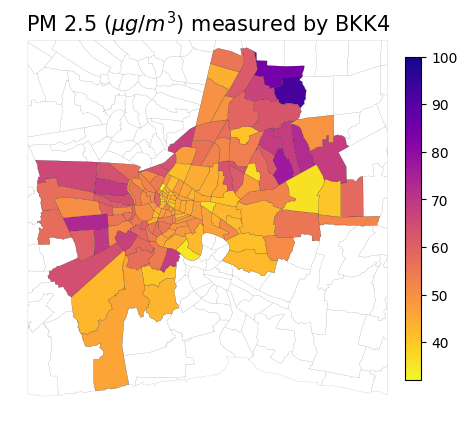
\includegraphics[width=.49\linewidth]{figures/map/BKK4_PM25.png}%
        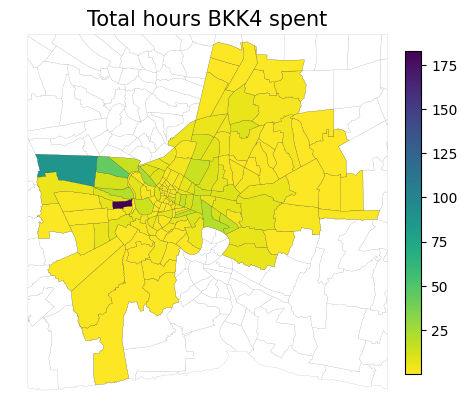
\includegraphics[width=.49\linewidth]{figures/map/BKK4_time.png}
        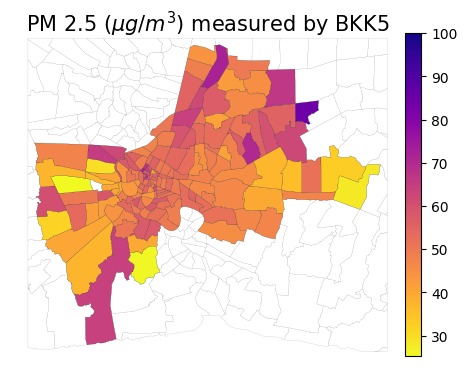
\includegraphics[width=.49\linewidth]{figures/map/BKK5_PM25.png}%
        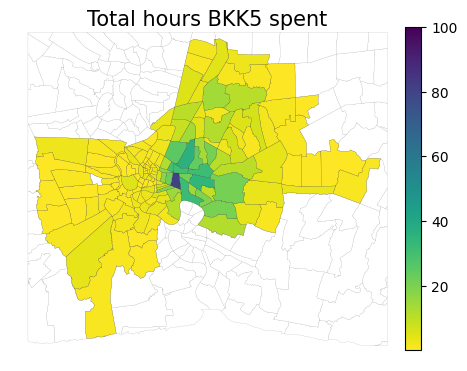
\includegraphics[width=.49\linewidth]{figures/map/BKK5_time.png}
        \caption{Measurement collected in Bangkok.}
        % \label{fig:hourly-work-aqi}
    \end{subfigure}%
    \hfill%
    \begin{subfigure}[t]{0.49\textwidth}
        \centering
        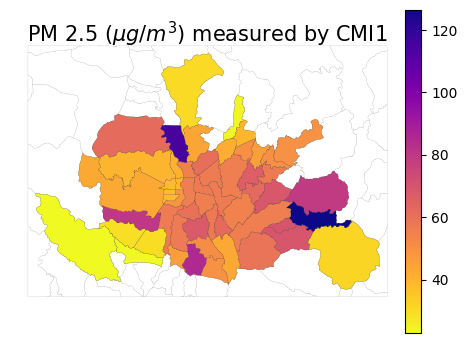
\includegraphics[width=.49\linewidth]{figures/map/CMI1_PM25.png}%
        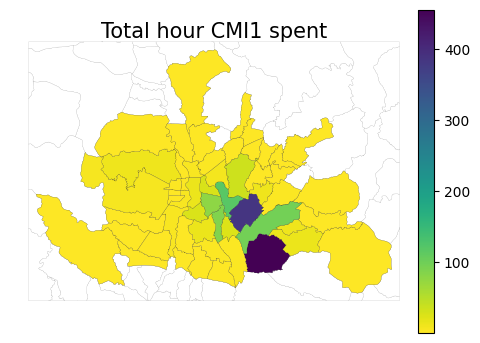
\includegraphics[width=.49\linewidth]{figures/map/CMI1_time.png}
        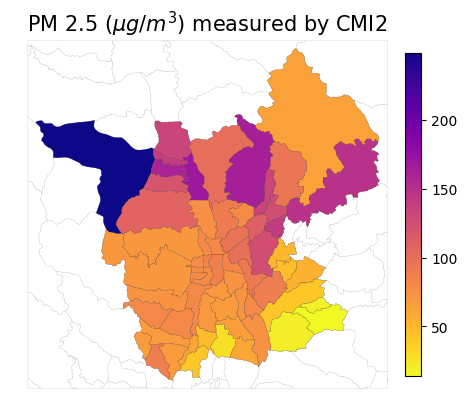
\includegraphics[width=.49\linewidth]{figures/map/CMI2_PM25.png}%
        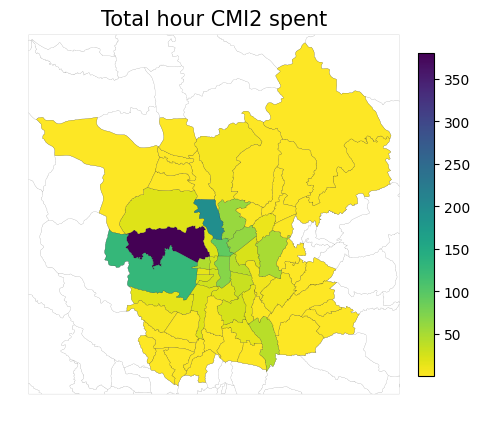
\includegraphics[width=.49\linewidth]{figures/map/CMI2_time.png}
        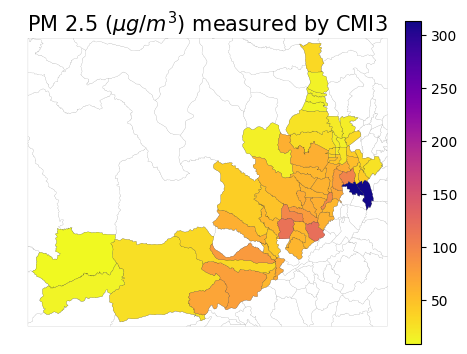
\includegraphics[width=.49\linewidth]{figures/map/CMI3_PM25.png}%
        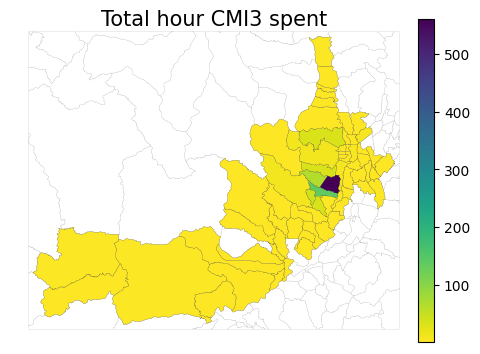
\includegraphics[width=.49\linewidth]{figures/map/CMI3_time.png}
        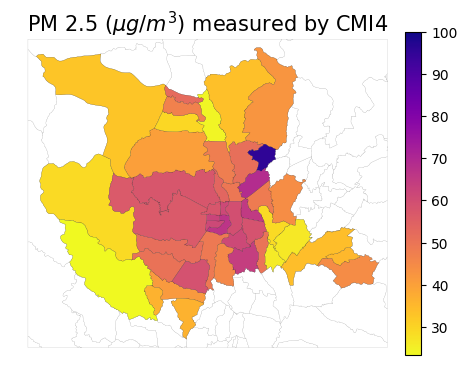
\includegraphics[width=.49\linewidth]{figures/map/CMI4_PM25.png}%
        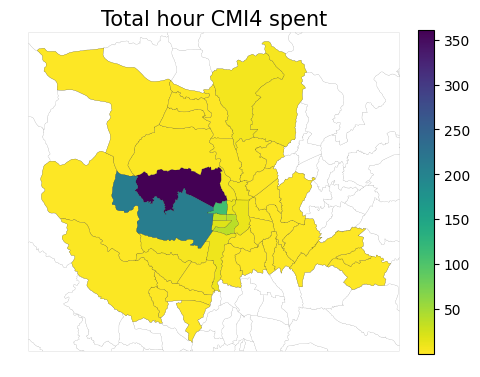
\includegraphics[width=.49\linewidth]{figures/map/CMI4_time.png}
        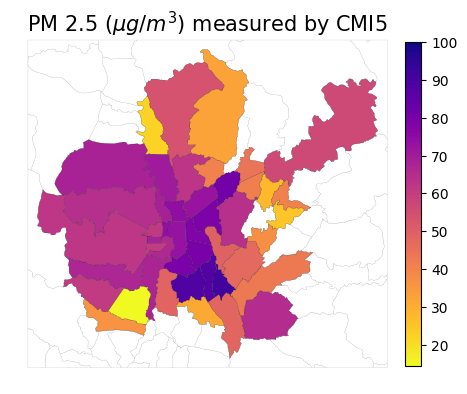
\includegraphics[width=.49\linewidth]{figures/map/CMI5_PM25.png}%
        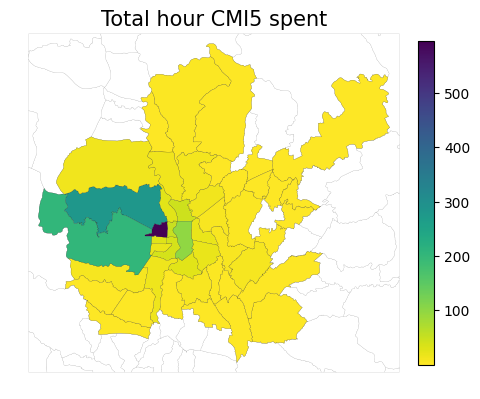
\includegraphics[width=.49\linewidth]{figures/map/CMI5_time.png}
        \caption{Measurement collected in Chiang Mai.}
        % \label{fig:hourly-work-hours}
    \end{subfigure}%
    \caption{
    % \joe{wait... the color bars are all wildly different on these plots lol. you can't even compare between them...}
    The left column of each sub-figure shows the average PM2.5 level throughout the study period measured in each subdistrict.
    The right column of each sub-figure shows the amount of time in hours that each driver spent in each subdistrict throughout the study.
    % \mick{todo: shared color axis?}
    % \mick{todo: same vis sizes}
    % \mick{todo: use latex notation for units}
    % \mick{todo: include all the subdistricts}
    % \joe{Shall we lower the opacity of the districts where there is no data at all in the left plots? based on the right plot, I can't tell if the purple districts have 0 hours spent or a very small amount of hours spent. If it is 0, I don't want to see measurements in the left plot. Maybe every person spent time in every district so if we want to make this more clear, just do a log plot in color dimension.}
    }%
    \Description{}
    \label{fig:subdistrict-aqi}%
\end{figure*}%

% \input{sections/4-2-systemic-3-response}
\subsection{Driver Responses to Air Pollution Exposure}
This section explores how drivers responded to the observed air pollution patterns, combining quantitative findings with qualitative insights from interviews and driver archetypes (``Income-Driven'' and ``Health-Conscious'').
While quantitative analysis reveals complex exposure patterns varying temporally (\autoref{fig:daily-pollution-per-driver}, \autoref{fig:hourly-work-aqi}) and spatially (\autoref{fig:subdistrict-aqi}) across individuals and cities,
driver responses show limited adaptation, dictated primarily by economic needs and the perceived unavoidability of pollution.

\subsubsection{Prioritizing Income Amidst Pervasive Pollution}
Our analysis reveals no correlation between drivers' daily work hours and concurrent average PM2.5 levels (\autoref{fig:work-hours-vs-aqi-per-rider}), indicating a lack of temporal work adjustments in response to pollution fluctuations.
This aligns with qualitative interviews where drivers frequently expressed perceiving pollution exposure as an unavoidable occupational hazard rather than a modifiable risk.
Many prioritized immediate income over avoiding polluted times, echoing sentiments like,

\qpadding
\fcolorbox{gray}{white}{%
  \begin{minipage}{.9\linewidth} \em
``I just go where the application tells me to go, ..., the (air) pollution is everywhere anyway.'' (BKK1)
  \end{minipage}
}

\qpadding
\fcolorbox{gray}{white}{%
  \begin{minipage}{.9\linewidth} \em
    ``When I see that the area gets smoggier, I often thought about driving out to the suburban area. But that means I'll have to drive an empty car out.'' (BKK5)
   \end{minipage}
}
\qpadding

This ``Income-Driven'' approach was common.
Driver BKK1 (46, Male), targeting 2,000-2,500 baht daily through long hours (4 AM-9 PM), exemplified this.
Despite experiencing symptoms like runny noses and eye irritation and becoming aware of pollution levels via our map visualization after joining the study, his driving patterns remained unchanged.
He explained his reliance on masks and persistence:

\qpadding
\fcolorbox{gray}{white}{%
  \begin{minipage}{.9\linewidth} \em
    ``I can feel my body gets weaker (the more I drive); I always wear masks. ... If Google Maps tells us to go, I go. Wherever it is, I just have to push through.'' (BKK1)
  \end{minipage}
}
\qpadding

He further emphasized the lack of choice dictated by the platform and financial needs:

\qpadding
\fcolorbox{gray}{white}{%
  \begin{minipage}{.9\linewidth} \em
    ``I will not be able to be selective about routes; I go wherever the application assigns me to go, no matter of how far or how polluted the area may be.'' (BKK1)
  \end{minipage}
}
\qpadding

% This practice, where enduring poor air is ``simply something they have to be able to live with'' (BKK-4), mirrors observations in gig work research regarding the normalization of health risks under precarious conditions.

% \begin{quoteb}
%     ``People who choose to become (motorcycle taxi) drivers, they know what they get themselves into. Pushing through rains or pollution is simply just something they have to be able to live with.'' (BKK-4)
% \end{quoteb}

% While drivers do not adjust work schedules, spatial analysis reveals they spend the majority of their time in subdistricts with relatively lower PM2.5 levels (below 100 $\mu g / m^3$, often below 50 $\mu g / m^3$).
% This suggests some passive or possibly active spatial avoidance, perhaps by choosing service areas known anecdotally to be less polluted, even if not actively avoiding specific high-pollution zones on a trip-by-trip basis.
The dominant narrative remains that immediate economic needs override pollution avoidance strategies concerning work timing.

\subsubsection{Limited Mitigation}
While prioritizing income was dominant, some drivers, exemplified by the ``Health-Conscious'' driver BKK3, attempted mitigation strategies within existing constraints.
BKK3 (54, Female) actively incorporated heightened air pollution awareness into driving decisions after using the sensor helmet and map visualization.
She observed pollution spikes when riding behind buses,

\qpadding
\fcolorbox{gray}{white}{%
  \begin{minipage}{.9\linewidth} \em
    ``When I follow big buses, the graph just shoots up immediately.'' (BKK3)
  \end{minipage}
}
\qpadding
% \begin{quoteb}
%     ``When I follow big buses, the graph just shoots up immediately.'' (BKK3)
% \end{quoteb}

and gained insight into hazardous AQI levels (80-100 \textmu{}g/m$^3$) even on seemingly clear days. This awareness prompted actions like avoiding main roads for side streets, despite potentially longer distances,

\qpadding
\fcolorbox{gray}{white}{%
  \begin{minipage}{.9\linewidth} \em
    ``Main roads have more dusts (air pollutants), it’s better to go through small alleys.'' (BKK3)
  \end{minipage}
}
\qpadding

and selectively accepting rides or disabling auto-matching nearby to reduce prolonged exposure, particularly when heading home.

% However, complete avoidance was impossible due to passenger demand and platform algorithms.
% Physical symptoms (nasal irritation, dry throat) sometimes led her to finish work early,
% \begin{quoteb}
%     ``I go home earlier quite often when I feel my nose stings and my throat feels dry.'' (BKK-3)
% \end{quoteb}

% Moreover, immediate safety threats like rain were prioritized over pollution concerns \cite{tieanklin2024rideshare}.
However, despite finding the real-time, localized AQI data useful, financial needs prevailed:

\qpadding
\fcolorbox{gray}{white}{%
  \begin{minipage}{.9\linewidth} \em
    ``We took this job for the money. We just have to live with it.'' (BKK3)
  \end{minipage}
}
\qpadding

BKK3's experience illustrates the tension between health awareness and economic necessity.
% , highlighting the limited scope for individual mitigation.
While information tools provide valuable insights, platform constraints significantly limit drivers' ability to act on this information without sacrificing income.

In this study, we do not observe a correlation between drivers' mitigation behaviors and their age or gender.

\subsubsection{Increased Awareness and Community Engagement}
Participation in the study and access to the map visualization significantly increased drivers' awareness and spurred public engagement.
Most participants reported frequently checking the visualization, particularly on high-pollution days.
This led to discussions about air quality with friends and passengers; for instance, CMI4 advised others on mask use, while BKK4 shared real-time data from the visualization with passengers during rides in poor conditions.
The visualization thus served both as a personal reference tool and a catalyst for community awareness.

Driver CMI1 exemplified proactive community engagement.
He monitored morning pollution levels and actively shared warnings in the Chiang Mai rideshare driver community (>5,000 members) when conditions were hazardous:

\qpadding
\fcolorbox{gray}{white}{%
  \begin{minipage}{.9\linewidth} \em
 ``I often take a screenshot (of the map visualization) when the air pollution levels turn red (hazardous) and share it in the group, warning everyone to be extra careful since the pollution got worsen that day.'' (CMI1)
  \end{minipage}
}
\qpadding

This demonstrates how access to real-time, localized data empowered drivers beyond personal monitoring.
It fostered collective awareness and turned some participants, like CMI1, into informal educators and active contributors to environmental health knowledge sharing within their community, moving beyond passive data reception.

\begin{figure*}
    \centering
    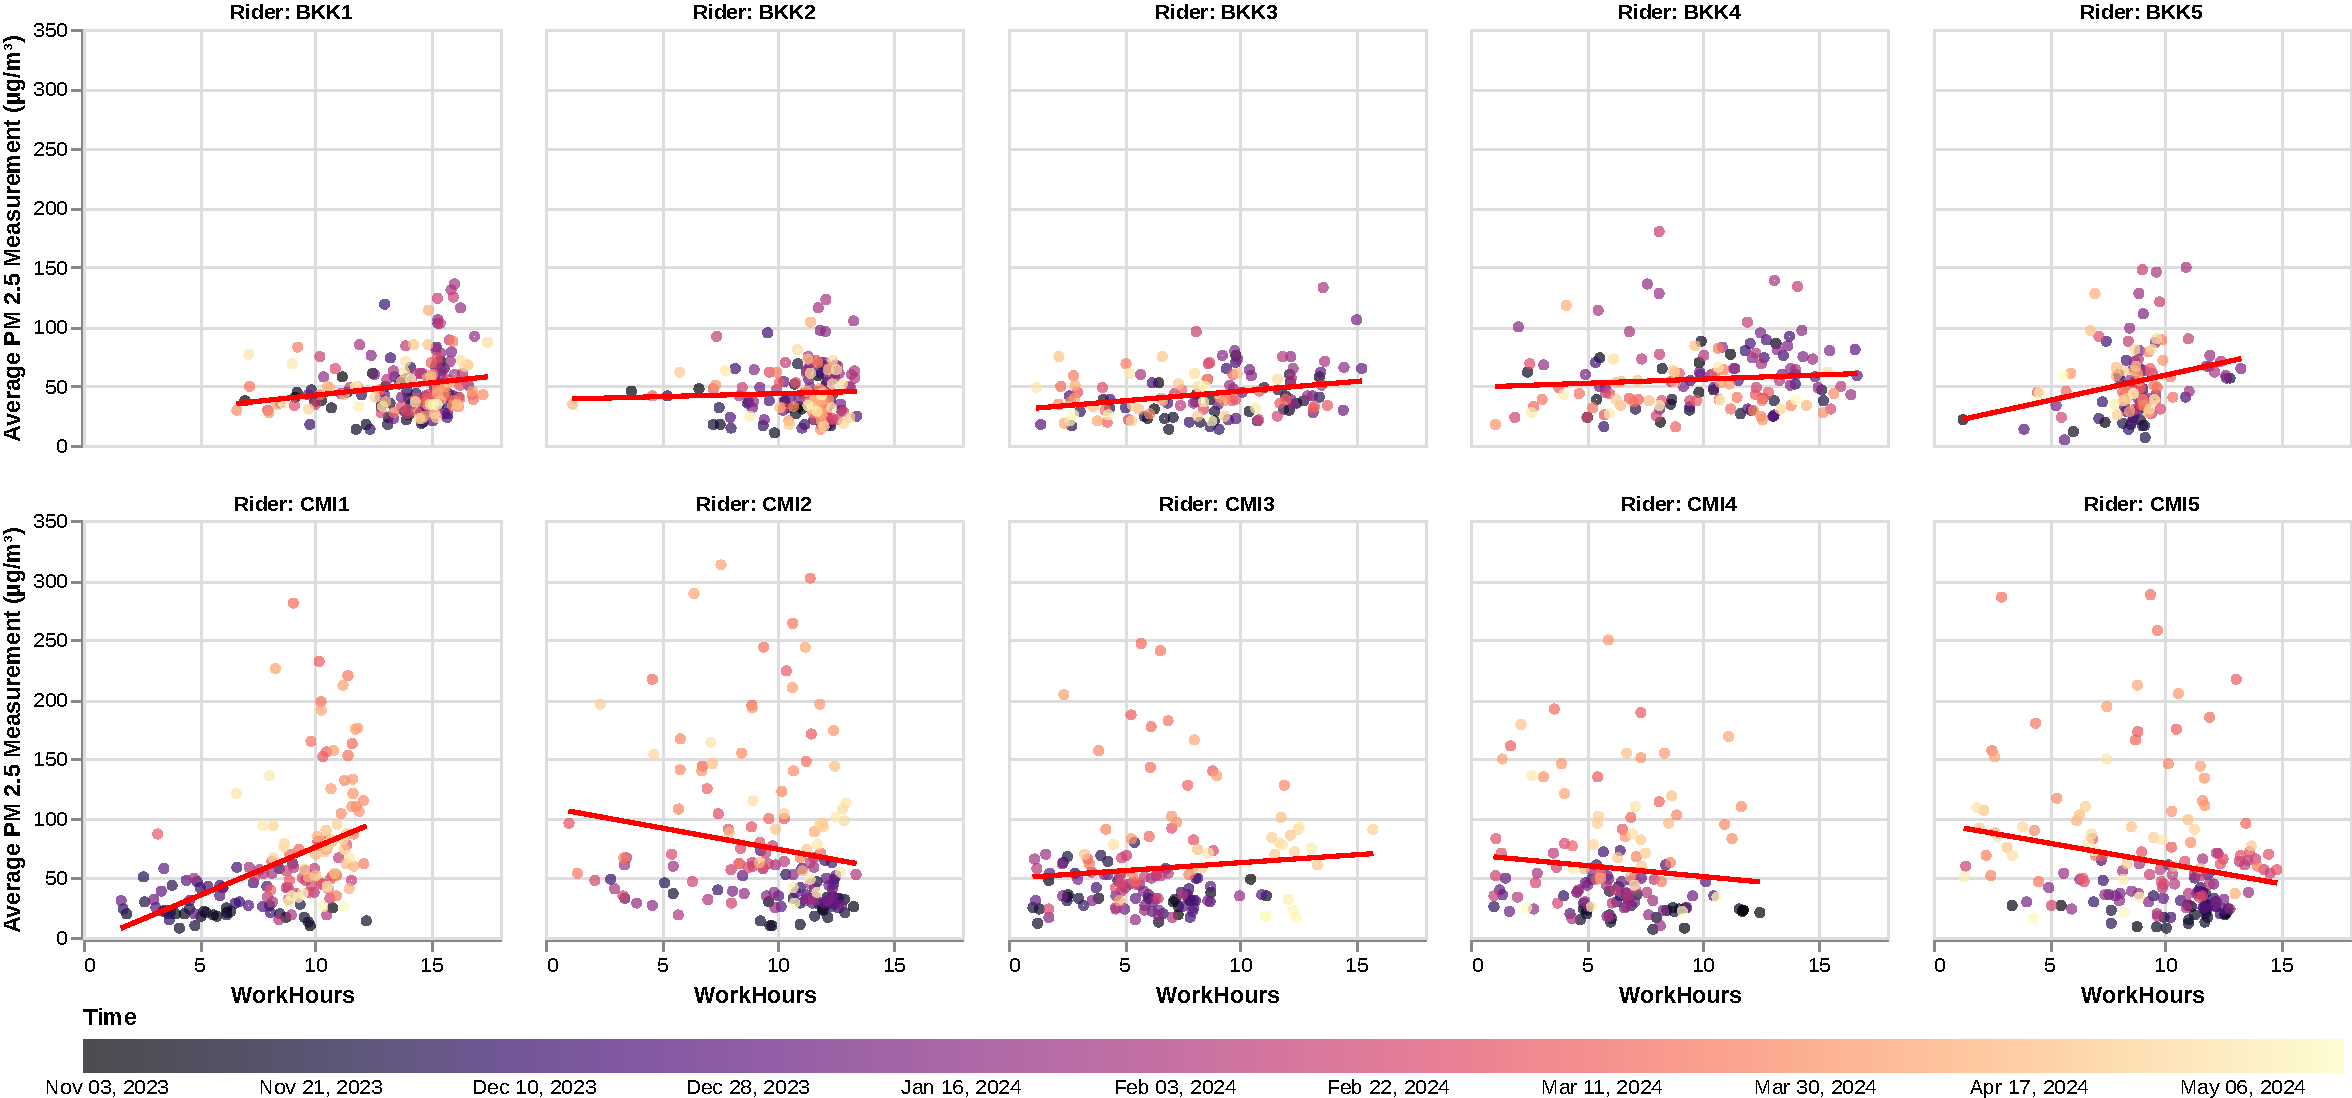
\includegraphics[width=\textwidth]{figures/work-hours-vs-aqi-per-rider-regression.pdf}
    \caption{Correlation of daily work hours and air pollution measurement for each driver, averaged through each week, with regression lines.
    % \joe{why are we aggregating to a weekly scale if we have daily data? A scatterplot is literally the perfect opportunity to represent disaggregated data and based on the fact that so many plots in this paper are per-participant, it seems like you wnat to show as fine grained data as possible?}
    }
    \Description{}
    \label{fig:work-hours-vs-aqi-per-rider}
\end{figure*}

Overall, while access to air quality information increased awareness and even spurred community engagement, the demanding nature of gig work and the perceived ubiquity of pollution limit drivers' capacity to translate this awareness into significant behavioral changes, particularly regarding work schedules.
Financial imperatives largely override health considerations, highlighting the need for systemic interventions beyond individual information provision to effectively reduce exposure, such as low-emission zones or integrating real-time AQ data into traffic management.
% \input{sections/4-3-individual}
% \subsection{Communal Engagement -- From Technical Support to a Community Space}
\label{sec:result-communal-engagement}
% Group Interactions and Air Quality Discourse

In this subsection, we explore how motorcycle taxi drivers in Bangkok and Chiang Mai engaged in collective sensemaking through their group chat interactions, leveraging air quality data from their sensors. 

\subsubsection{Sense of Community and Social Support}
Initially created as a technical support channel, the group chat quickly evolved into a vital community space where drivers from both provinces, Bangkok and Chiang Mai, shared their day-to-day driving experiences, unexpected circumstances, traffic congestion and most importantly, warned each other about worsening air pollution conditions in their respective areas.  

During peak pollution days, the chat became particularly active, with drivers providing real-time updates. On December 11, 2024, one of the first major pollution waves of the season in Bangkok, driver BKK-5 began their day by checking the air quality web portal that we provided and alerting everyone in the groupchat,

\begin{quoteb}
    ``Today the air pollution is really thick, it's very red.'' (BKK-5)
\end{quoteb}

\mick{can remove this paragraph because does not make the point for the communal engagement.}
BKK-5 Driver also reported during the exit interview that he often checked the map visualization showing the air pollution level every day and constantly checked for updates throughout the day, especially during the peak period in January and February.

Beyond leveraging the data that they have collectively collected, the group chat functioned as a space for social support, where drivers expressed concerns about health risks and reminded other participants, sometimes the research team included, to prepare protective measures mitigating exposure. 
This illustrates how the integration of sensor data into social communication channels can enhance risk awareness and foster a sense of community among participants.


\subsubsection{Shared Situational Awareness and Collaborative Interpretation}
Beyond warnings, drivers also used the visualization tools to compare pollution levels between the two cities, Bangkok and Chiang Mai, fostering a shared understanding of exposure risks. 
% Some expressed concerns about their peers’ conditions, reinforcing a sense of solidarity despite being geographically apart.
Our participants reported developing a new habit of frequently checking both their own and other participants' air quality measurements using the map visualization web application, particularly during downtime while waiting for the next ride request.
For instance, BKK-4 was the first to notice the onset of one of the worst air pollution waves in Chiang Mai of 2024, where sensor data showed PM2.5 levels exceeding 200 $\mu g/m^3$ during the day. BKK-4 remarked,

\begin{quoteb}
``(Air pollution in) Chiang Mai has been getting a lot worse a lot lately.'' (BKK-4)
\end{quoteb}

Drivers often use the visualization web application not only to navigate their immediate environment but also to stay informed about broader regional trends.

This emergent community dynamic highlights that drivers are not indifferent to air pollution risks; rather, as discussed earlier, they perceive it as an unavoidable part of their job. Given that motorcycle taxi driving is their primary source of income, individual avoidance strategies remain limited, further underscoring the need for broader structural interventions. 

\subsubsection{Leverage The Tool for Income}
Drivers frequently utilize the air quality map to identify ``red'' zones, which indicate high pollution levels, and infer traffic congestion in those areas. This capability allows them to strategize their routes to maximize income by avoiding congested areas while simultaneously minimizing exposure to poor air quality. 
The interviews with drivers have revealed the dual benefits of using the map visualization web application - optimizing income by increasing the number of pickups while also subsequently  reducing the health risks from the air pollutions as they would just avoid the area.
For instance, one of the most-earning Bangkok drivers noted during the exit interview,

\begin{quoteb}
``It will actually be even more helpful to actually show the traffic real-time, so I can avoid the area altogether...  I can make more rounds of pickups and also reduce the air pollution intake too.'' (BKK-5)
\end{quoteb}


The drivers’ ability to interpret air quality data in conjunction with traffic conditions reflects a strategic approach to their work, where financial incentives take precedence over health considerations. 
This aligns with the previous research for this particular group indicating that gig workers often prioritize immediate income due to precarious employment conditions, leading them to overlook long-term health implications \cite{tieanklin2024rideshare, zhang2022algorithmic}. 
This underscores the need for targeted interventions that address both economic and health concerns for gig workers in urban environments.